\documentclass[a4paper]{article}
\usepackage[utf8]{inputenc}
\usepackage{graphicx,tikz,hyperref,booktabs,lmodern,textcomp,multirow,microtype}
\usetikzlibrary{shapes,positioning,calc}

\title{Audio Mixer}
\author{Patrick M. Elsen}
\date{\today}

\renewcommand{\arraystretch}{1.2}

\newenvironment{partdisplay}[1]{
\begin{center}
\begin{tabular}{@{}p{3cm}p{3cm}p{4.5cm}@{}}
\multirow{2}{3cm}{\includegraphics[width=3cm]{images/#1}}}{
\end{tabular}
\end{center}}

\begin{document}
\maketitle
\tableofcontents

\section{Introduction}

In this project, I attempt to build an audio mixer. This is a device that I need for myself, and have needed for a while. 

My background is in IT. I don't really have any formal training in electronics engineering but find the subject to be very fascinating. I expect to make some mistakes or come up with designs that are maybe suboptimal or too expensive, but that is acceptable.

\section{Specifications}

\begin{figure}[!h]
\centering  
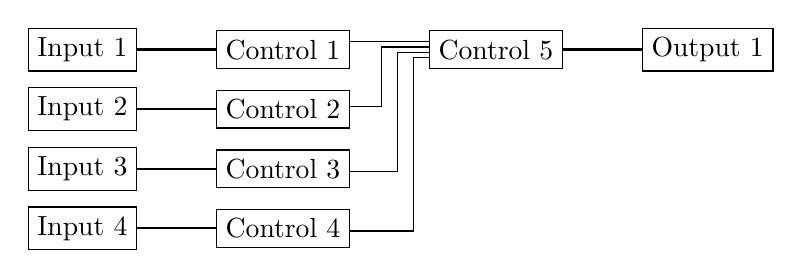
\begin{tikzpicture}
\node[rectangle,draw] (input1) {Input 1};
\node[below=2mm of input1,rectangle,draw] (input2) {Input 2};
\node[below=2mm of input2,rectangle,draw] (input3) {Input 3};
\node[below=2mm of input3,rectangle,draw] (input4) {Input 4};
\node[right=1cm of input1,rectangle,draw] (control1) {Control 1};
\node[right=1cm of input2,rectangle,draw] (control2) {Control 2};
\node[right=1cm of input3,rectangle,draw] (control3) {Control 3};
\node[right=1cm of input4,rectangle,draw] (control4) {Control 4};
\draw[thick] (input1) -- (control1);
\draw[thick] (input2) -- (control2);
\draw[thick] (input3) -- (control3);
\draw[thick] (input4) -- (control4);
\node[right=1cm of control1,rectangle,draw] (control5) {Control 5};
%\node[right=1cm of control2,rectangle,draw] (control6) {Control 6};
\draw ([yshift=1mm]control1.east) -- ++(0.2,0) |-([yshift=1mm]control5.west);
\draw ([yshift=0.33mm]control2.east) -- ++(0.4,0) |-([yshift=0.33mm]control5.west);
\draw ([yshift=-0.33mm]control3.east) -- ++(0.6,0) |-([yshift=-0.33mm]control5.west);
\draw ([yshift=-0.33mm]control4.east) -- ++(0.8,0) |-([yshift=-1mm]control5.west);
\node[right=1cm of control5,rectangle,draw] (output1) {Output 1};
%\node[right=1cm of control6,rectangle,draw] (output2) {Output 2};
\draw[thick] (control5) -- (output1);
%\draw[thick] (control6) -- (output2);
\end{tikzpicture}
\caption{Logic diagram of audio mixer}
\end{figure}

\begin{enumerate}
  \item Takes power from USB or 12V input jack (either one is fine, USB would be nice).
  \item Takes four stereo inputs, ideally as RCA jacks.
  \item Has volume controls for each of the inputs.
%  \item Has two separate volume outputs.
  \item Has a master volume control.
  \item Optionally, a second output channel (with an independent volume control).
%  \item Has independent master volume controls for each of the outputs.
  \item Based on the LF353 operational amplifier.
  \item Has to fit on a 10x10cm PCB at max for cheapest production costs.
\end{enumerate}

I came up with these specifications because this is what I need: I have multiple devices on my desk, including my desktop Mac Mini, my MacBook Pro, occasionally another laptop and my phone. Each of these devices should be able to send audio to my stereo system, but my stereo is very basic and has only one line-level input.

This device needs to be able to take audio from any of my devices, mix it together, and send it to either my stereo or my headphones. It does not need to do any amplification.

I chose the LF353 because it is available in a small but convenient form factor and relatively inexpensive. Also, SeeedStudio has it in stock.

\section{Research}

I did a bit of research while coming up with the specifications. I need to use some software to actually design the schematic and PCB. I also need to source parts, produce the PCB, and assemble the PCB.

\begin{enumerate}
  \item KiCAD (\url{http://www.kicad-pcb.org/}) is my tool of choice for PCB design.
  \item SnapEDA (\url{https://www.snapeda.com/}) has part outlines and models for KiCAD and is free to use.
  \item SeeedStudio (\url{https://www.seeedstudio.com/}) offers PCB manufacture, assembly, and parts that I might use.
\end{enumerate}

It is important that I find good connectors and potentiometers that will last a while. For the case, I will find ideas after I have designed the PCB, since it is easy to 3D-print a case.

\section{Parts}

\subsection{RCA Connector}

I need five sets of two RCA connectors (one connect for each of the two stereo channel for every input and output, with four inputs and one output, that makes five). I browsed DigiKey for the most rubust and yet cost-effective option, and found a number of candidates.

The important criterions were  that it is stocked (such that I can order the parts and expect them within a reasonable time frame).

At first, I found a simple two-contact RCA input. With the discounted rate by ordering at least ten, this part would cost 5.40€ for all five channels. That is quite a bit more expensive that I had thought it would be.

\begin{center}
\begin{tabular}{@{}p{3cm}p{3cm}p{3cm}@{}}
%\toprule
\multirow{2}{3cm}{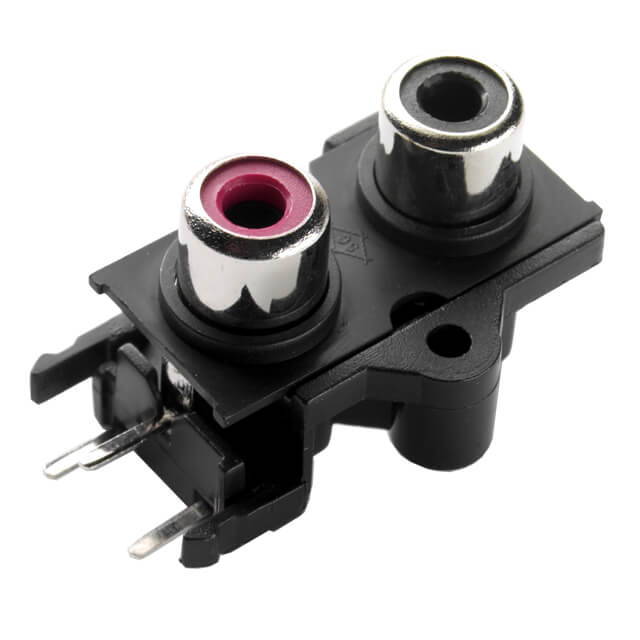
\includegraphics[width=3cm]{images/MFG_RCJ-22}}
& DigiKey Part & 102-5864-ND\\
& Manufacturer & CUI Devices\\
& Manufacturer Part & RCJ-2233\\
& Contacts & 2\\
& Price (1) & 1.23€\\
& Price (10) & 1.08€\\
%\bottomrule
\end{tabular}
\end{center}

Next, I was looking for bigger parts, thinking that it might potentially save money to buy larger. The one I found I thought looks really nice, with the metal and golden contacts. However, it does not seem to be cheaper than just using two simple 2-channel ones.

\begin{center}
\begin{tabular}{@{}p{3cm}p{3cm}p{3cm}@{}}
%\toprule
\multirow{2}{3cm}{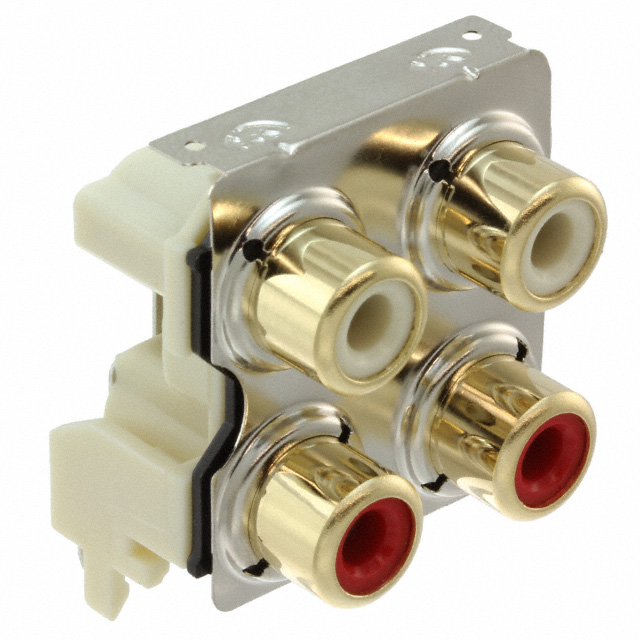
\includegraphics[width=3cm]{images/PJRAS2X2S01AUX}}
& DigiKey Part & SC2888-ND\\
& Manufacturer & Switchcraft Inc.\\
& Manufacturer Part & PJRAS2X2S01X\\
& Contacts & 4\\
& Price (1) & 2.88€\\
& Price (10) & 2.76€\\
%\bottomrule
\end{tabular}
\end{center}

When looking for even bigger ones, it seems like I found the one. An 8-input one that will do for all of the four stereo inputs, at only 3.79€.

\begin{center}
\begin{tabular}{@{}p{3cm}p{3cm}p{3cm}@{}}
%\toprule
\multirow{2}{3cm}{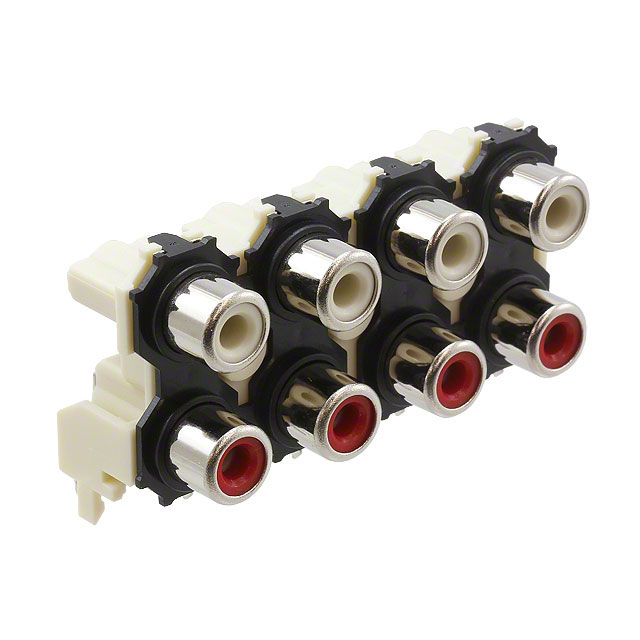
\includegraphics[width=3cm]{images/PJRAS4X2U01X}}
& DigiKey Part & SC1537-ND\\
& Manufacturer & Switchcraft Inc.\\
& Manufacturer Part & PJRAS4X2U01X\\
& Contacts & 8\\
& Price (1) & 3.79€\\
& Price (10) & 3.63€\\
%\bottomrule
\end{tabular}
\end{center}

\subsection{Opamps}

I need at least 10 opamps for the design that I have in mind -- one for every channel of the input (for 8 channels in total), plus one for every channel of the outputs (for an additional 2 channels).

The specifications state that I want to use the LF353 operational amplifier, however this is not a hard requirement. It is acceptable for me to use any other kind, as long as it is cheap, deliverable and works for audio applications. I exclude BGA parts from the search because I don't want to have too much issues in soldering them.

The prices I list here are the DigiKey prices, but I might end up sourcing them from SeeedStudio due to their assembly offer. 

\begin{center}
\begin{tabular}{@{}p{3cm}p{3cm}p{3cm}@{}}
%\toprule
\multirow{2}{3cm}{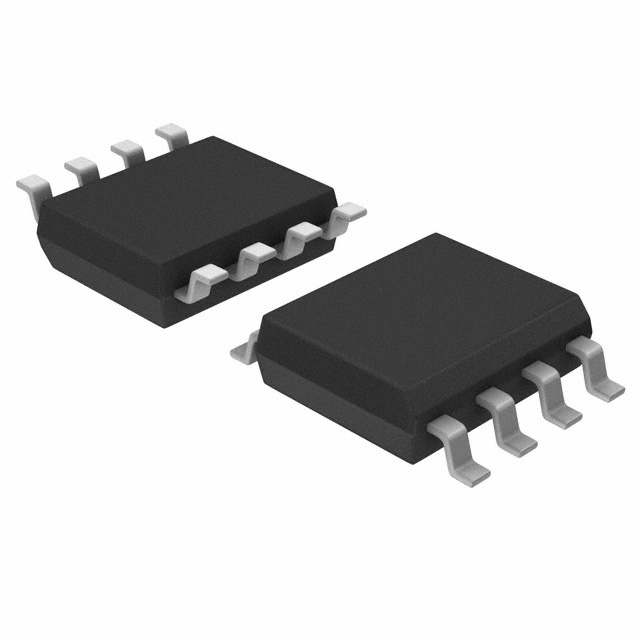
\includegraphics[width=3cm]{images/soic8}}
& DigiKey Part & 497-2967-1-ND\\
& Manufacturer & STMicroelectronics\\
& Manufacturer Part & LF353DT\\
& Opamps & 2\\
& Price (1) & 0.53€\\
& Price (10) & 0.44€\\
%\bottomrule
\end{tabular}
\end{center}

This first offer that I found is the one I was originally thinking about. It is offered by SeeedStudio and is, according to a single Google search, suitable for audio.

\begin{center}
\begin{tabular}{@{}p{3cm}p{3cm}p{3cm}@{}}
%\toprule
\multirow{2}{3cm}{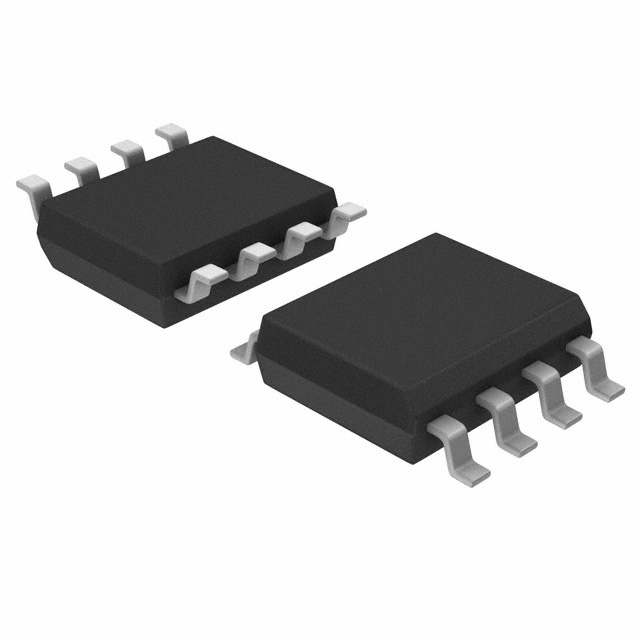
\includegraphics[width=3cm]{images/soic8}}
& DigiKey Part & 497-1597-1-ND\\
& Manufacturer & STMicroelectronics\\
& Manufacturer Part & LM833DT\\
& Opamps & 2\\
& Price (1) & 0.37€\\
& Price (10) & 0.31€\\
%\bottomrule
\end{tabular}
\end{center}

The second Opamp I found was one that is marked as being an amplifier specifically for audio on Digikey. The specs seem rather similar, I don't know what to make of most of them apart from the basics. But this one is cheaper, so I might go with it instead.

\begin{center}
\begin{tabular}{@{}p{3cm}p{3cm}p{3cm}@{}}
%\toprule
\multirow{2}{3cm}{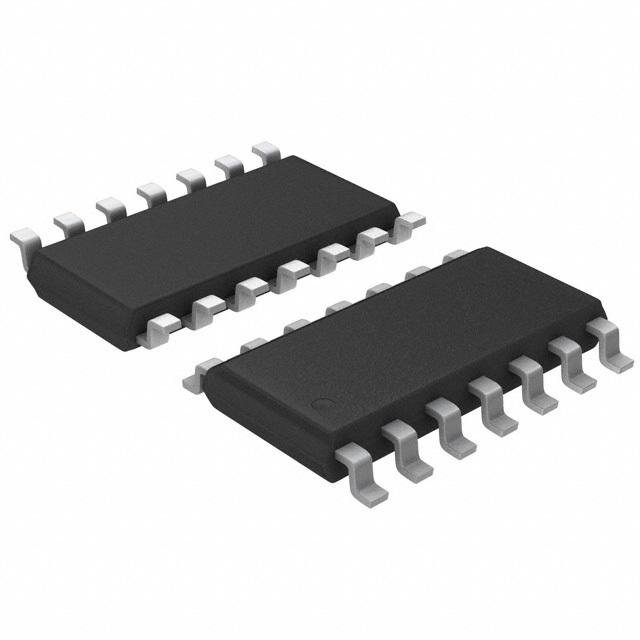
\includegraphics[width=3cm]{images/soic14}}
& DigiKey Part & 296-46621-1-ND\\
& Manufacturer & Texas Instruments\\
& Manufacturer Part & OPA1679IDR\\
& Opamps & 4\\
& Price (1) & 1.04€\\
& Price (10) & 0.88€\\
%\bottomrule
\end{tabular}
\end{center}

I also took a look at another operational amplifier with more channels. With the 2-channel opamps, I would need 5 ICs in total, which is maybe a bit much. Buying bigger packages means I can reduce the part count. This one is also suited to audio applications. However, it is more expensive than the LM833DT.

The main takeaway from the opamps is that I probably need a negative voltage rail. Ideally, I want something like a -12V and a +12V rail to give me a lot of headroom for the audio.

\subsection{Power Connector}

Choosing the right power connector is not an easy task. I have essentially two options.

\begin{itemize}
  \item Use a 12V barrel connector. This means I need an external power supply, which will cost additional money. However, this type of connector is ubiquitous, meaning that it will be easy to find parts. Also, power consumption like this is essentially unlimited.
  \item Use a USB connector. This might be more expensive. Also, power draw will be limited to 100mA unless I also use a chip to communicate to the other end that I need to draw more power. This will limit the voltage to 5V, meaning that I might need some logic to step up that voltage (and filter it to get a really clean supply).
\end{itemize}

I looked at both options to compare prices and see what is available. For the USB plug, I excluded USB type C due to the price as it is a newer standard.

\begin{partdisplay}{10118193-0001LF}
& DigiKey Part & 609-4616-1-ND\\
& Manufacturer & Amphenol ICC (FCI)\\
& Manufacturer Part & 10118193-0001LF\\
& Type & Micro USB\\
& Price (1) & 0.38€\\
& Price (10) & 0.36€\\
\end{partdisplay}

This first one I found I liked, it is inexpensive at 0.38€ and looks alright. I am a little worried about durability here, as these don't offer a clip to hold them down and provide extra strength.

\begin{partdisplay}{MFG_PJ-037A}
& DigiKey Part & CP-037A-ND\\
& Manufacturer & CUI Devices\\
& Manufacturer Part & PJ-037A\\
& Type & 2mm/5.5mm Barrel Jack\\
& Price (1) & 0.52€\\
& Price (10) & 0.48€\\
\end{partdisplay}

The second option I looked at is the ubiquitous barrel jack. This one is, as expected, a little bit more pricey. However, it does have the advantage of being able to deliver a lot of power easily.

\subsection{Power Supply}

Because line audio operates as AC with the neutral being grounded, and I need to build followers, I need a negative rail. There are different methods by which this can be achieved, the easiest way being a DC to DC converter. Since I don't need a lot of current, the easiest way here might also be the cheapest way.

\begin{partdisplay}{MFG_PDME1-S}
& DigiKey Part & 102-6321-ND\\
& Manufacturer & CUI Inc.\\
& Manufacturer Part & PDME1-S5-D9-S\\
& Input & 4.5-5.5V\\
& Output & 9V, -9V\\
& Power & 56mA\\
& Price (1) & 2.19€\\
& Price (10) & 2.15€\\
\end{partdisplay}

The first part I found looks very promising already. It takes in USB level voltage, and is able to deliver a ±9V power rail. It is only able to deliver 56mA, which should however be enough for the opamps. The only issue with it is the price — at 2.19€, it is a very expensive part. This part is also available in a ±12V version at the same price.

I also took a look at some ICs that I might be able to use to generate the supply rails, but found that it was not really practical, as I would need to use two additional ICs along with support circuitry. I might look into this another time.

\subsection{Potentionmeters}

The potentiometers that I use in this product need to be of high quality such as not to degrade or introduce unwanted audible artefacts. Also, I probably want to use logarithmic ones, to give the audio control a more linear feel. Last, I need the potentionmeters to be dual-channel. When first looking, I forgot about that.

\begin{partdisplay}{PDB182}
& Digikey Part & PDB182-K425K-103A-ND\\
& Manufacturer & Bourns\\
& Manufacturer Part & PDB182-K425K-103A\\
& Resistance & 10k ±20\%\\
& Type & Logarithmic\\
& Power & 0.06W\\
& Price (1) & 1.71€\\
& Price (10) & 1.50€\\
\end{partdisplay}

This one looks like those really cheap Chinese potentiometers, but I guess that is just how potentiometers look like. I'm surprised at how expensive it is -- this would add 8€ towards the cost of the product. I hope I can find a more economical alternative. While looking for other potentiometers, I learned that there are many kinds of precision potentiometers, some selling for three-figure amounts.

I also consider whether it might be better for me to use linear regulators, since I happen to have some that I have not yet put to good use. Another consideration is maybe using a digital potentiometer rather than a physical one, and implementing some kind of control via the serial port. That would change the scope of the project a bit, and to be honest, I do like the idea of having a physical knob to turn. 

\begin{partdisplay}{EVJY}
& Digikey Part & P2J4103-ND\\
& Manufacturer & Panasonic Electronical Components\\
& Manufacturer Part & EVJ-YK6F03651\\
& Resistance & 10k ±20\%\\
& Type & Logarithmic\\
& Power & 0.05W\\
& Price (1) & 1.93€\\
& Price (10) & 1.19€\\
\end{partdisplay}

The second one I found is even more expensive -- at least when buying a single one. However, the price is acceptable when buying more than 10 at a time. It also has a good form factor.

\begin{partdisplay}{soic6}
& Digikey Part & MCP4018T-103E/LTCT-ND\\
& Manufacturer & Microchip Technology\\
& Manufacturer Part & MCP4018T-103E/LT\\
& Resistance & 10k\\
& Type & Linear\\
& Positions & 128\\
& Interface & I\textsuperscript{2}C\\
& Price (1) & 0.34€\\  
\end{partdisplay}

Just to know what that is all about, I also took a look at some digital potentiometers. The first one that I found looks really good at first glance -- especially the price looks good. However, upon further thinking, I realised that it is linear. It is possible to fake a logarithmic scale with a linear digital potentiometer, but that means that it would be limited to 7 audio positions, which doesn't sound all that great.

\begin{partdisplay}{175-16-QSOP}
& Digikey Part & MAX5456EEE+-ND\\
& Manufacturer & Maxim Integrated\\
& Manufacturer Part & MAX5456EEE+\\
& Resistance & 10k\\
& Type & Logarithmic\\
& Positions & 32\\
& Potentiometers & 2\\
& Interface & UP/DOWN Pins\\
& Price (1) & 3.05€\\
& Price (10) & 2.74€\\
\end{partdisplay}

Lastly, I found a chip that would actually work as a digital potentiometer. It is quite expensive, far more than the physical potentiometers, at 3€ per stereo channel. It would undoubtedly be fun to play with this and a microcontroller -- but it is out of the price range at this point.

\subsection{Capacitors}

As this deals with audio things, I need to make sure to use plenty good capacitors, as any type of noise will be noticeable. The datasheets of the components I use prescribe what kind of filter capacitors I need.

\begin{partdisplay}{nichion47cap}
& Digikey Part & 493-1808-ND\\
& Manufacturer & Nichicon\\
& Manufacturer Part & UPW1E4R7MDD\\
& Type & Electrolytic\\
& Capacity & 4.7µF\\
& Price (1) & 0.21€\\
& Price (10) & 0.14€\\  
\end{partdisplay}

The first cap I found is the one I will use for the filter caps on the input stage of the DC to DC transformer. It's surprisingly expensive to buy caps on digikey, normally they should be a couple cents a pop at most. All of this stuff adds to the BOM cost, which is a bit concerning.

\begin{partdisplay}{samsung8050}
& Digikey Part & 1276-1066-1-ND\\
& Manufacturer & Samsung Electro-Mechanics\\
& Manufacturer Part & CL21B105KAFNNNE\\
& Type & Electrolytic\\
& Capacity & 1µF\\
& Price (1) & 0.10€\\
& Price (10) & 0.07€\\  
\end{partdisplay}

The next cap I found is a ceramic cap. This is for power smoothing on the output of the DC to DC converter.

\begin{partdisplay}{samsung8050}
& Digikey Part & 1276-1014-1-ND\\
& Manufacturer & Samsung Electro-Mechanics\\
& Manufacturer Part & CL21C101JBANNNC\\
& Type & Electrolytic\\
& Capacity & 100pF\\
& Price (1) & 0.09€\\
& Price (10) & 0.05€\\  
\end{partdisplay}

\subsection{Inductors}

Since the datasheet of the DC to DC converter calls for an inductor on the input side, I looked for inductors. 

\begin{partdisplay}{MFG_MLZ2012}
& Digikey Part & 445-6402-1-ND\\
& Manufacturer & TDK Corporation\\
& Manufacturer Part & MLZ2012M6R8WT000\\
& Inductance & 6.8µH\\
& Current & 350mA\\
& Sat. Current & 220mA\\
& Price (1) & 0.13€\\
& Price (10) & 0.11€\\
\end{partdisplay}

This inductor is the first one I found. It has an acceptable price, so I went with it.

\subsection{Resistors}

I will likely also need a bunch of resistors -- however, I am not listing these here, as they are cheap enough that I don't need to worry about sourcing them.

\section{Design}

Next, I start my actual design process. I have downloaded and installed the most up-to-date version of KiCad on my system, which I will use to design this product. I have also made an account over at SnapEDA in order to access their free parts database. I start out with downloading all the parts I'm using or considering and import them into KiCad. I also downloaded and installed the Digikey library, but I was unable to find a lot of the parts I needed in it.

\subsection{USB Power Input}

The USB Power Input side was quite straightforward. I used the part for the USB connector. Since I don't actually do anything USB-related, I don't need to do anything with the data pins. All I do is tap off the V\textsubscript{in}, SHIELD and GND pins, and add a cap between the power rail and ground for filtering.

\begin{center}
  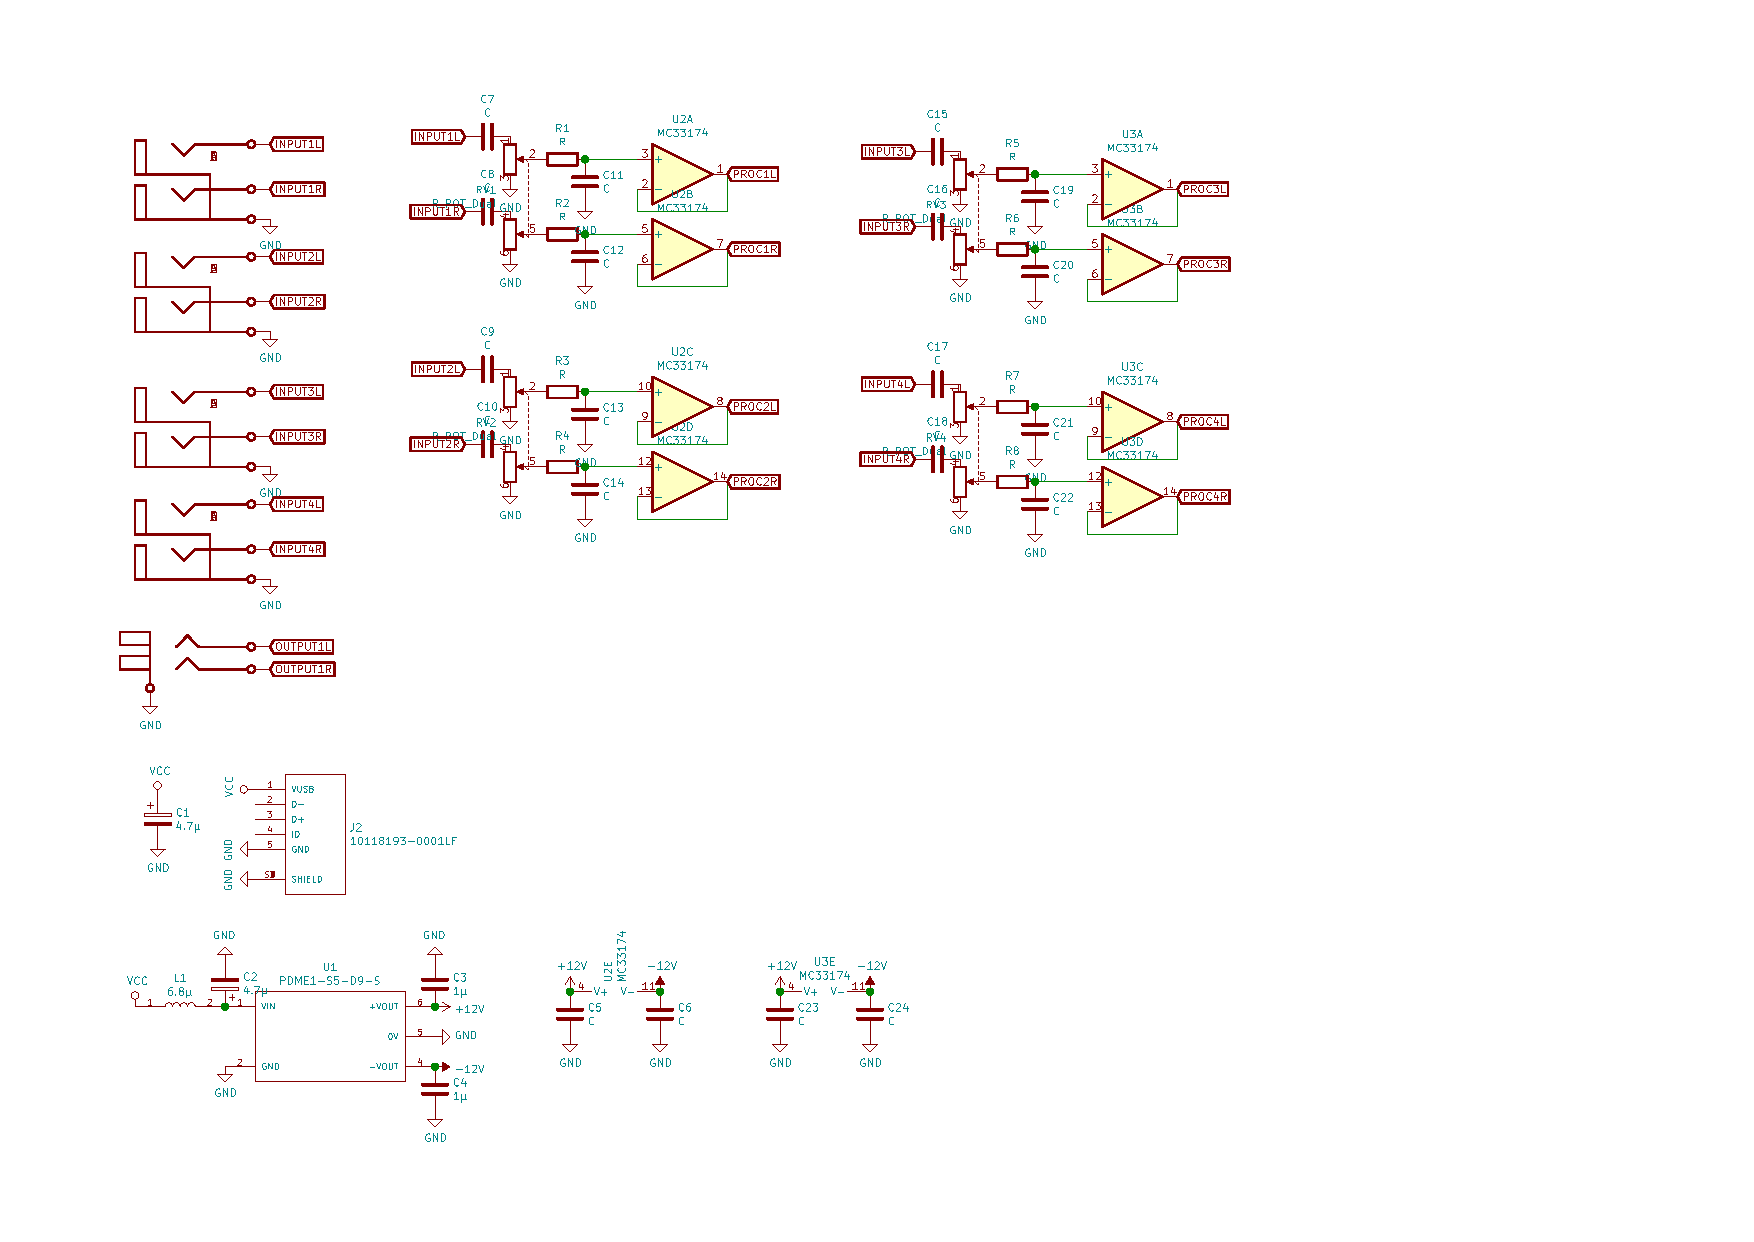
\includegraphics[trim={2cm 5.5cm 21cm 12.8cm},width=8cm,clip]{images/audio-mixer.pdf}
\end{center}

I might get back to this and add a fuse for protection, although I'm not sure yet if that is really necessary.

\subsection{Audio Input and Output}

For the audio inputs (RCA Jacks), I simply added all eight (four stereo channels) of them. I attached their ground to the common ground, and created labels for every one of them.

\begin{center}
  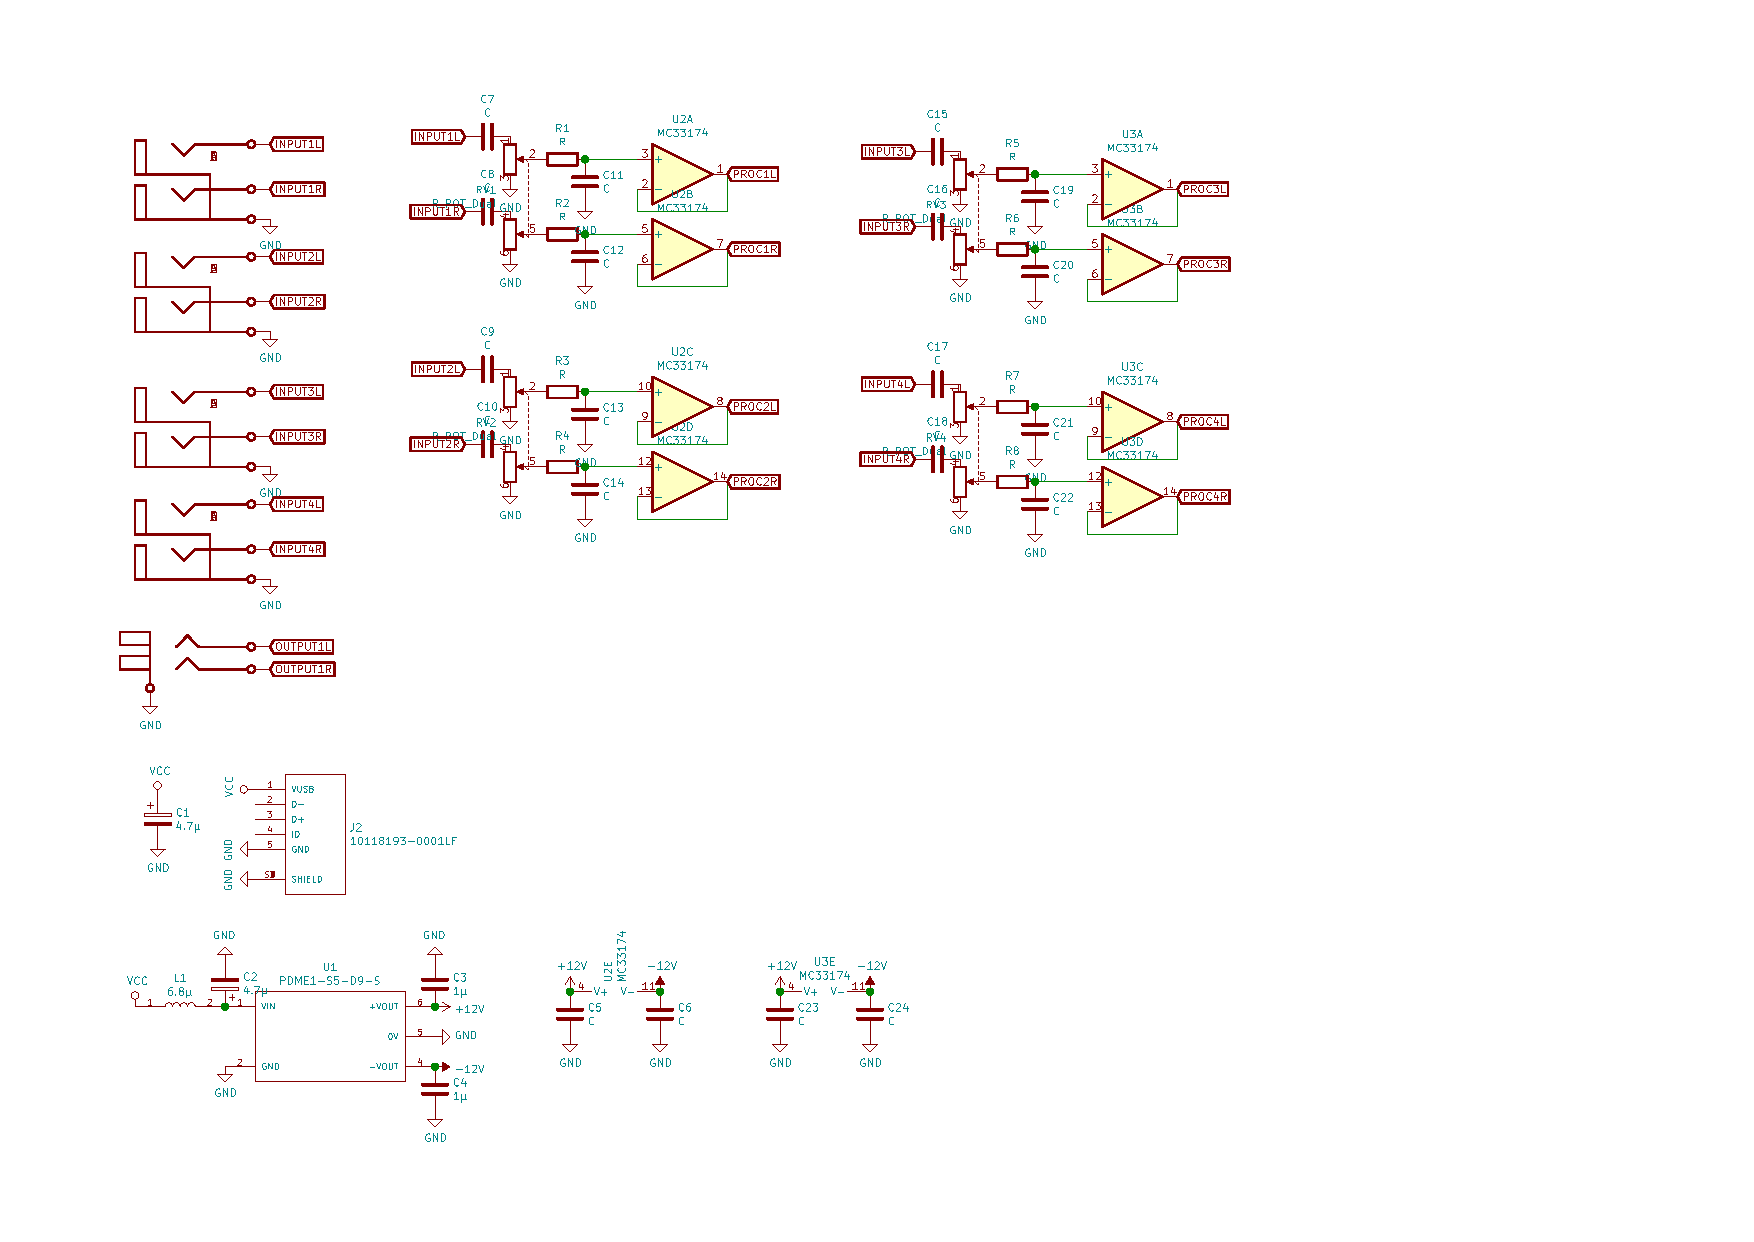
\includegraphics[trim={2cm 14.7cm 24cm 2cm},width=4cm,clip]{images/audio-mixer.pdf}
  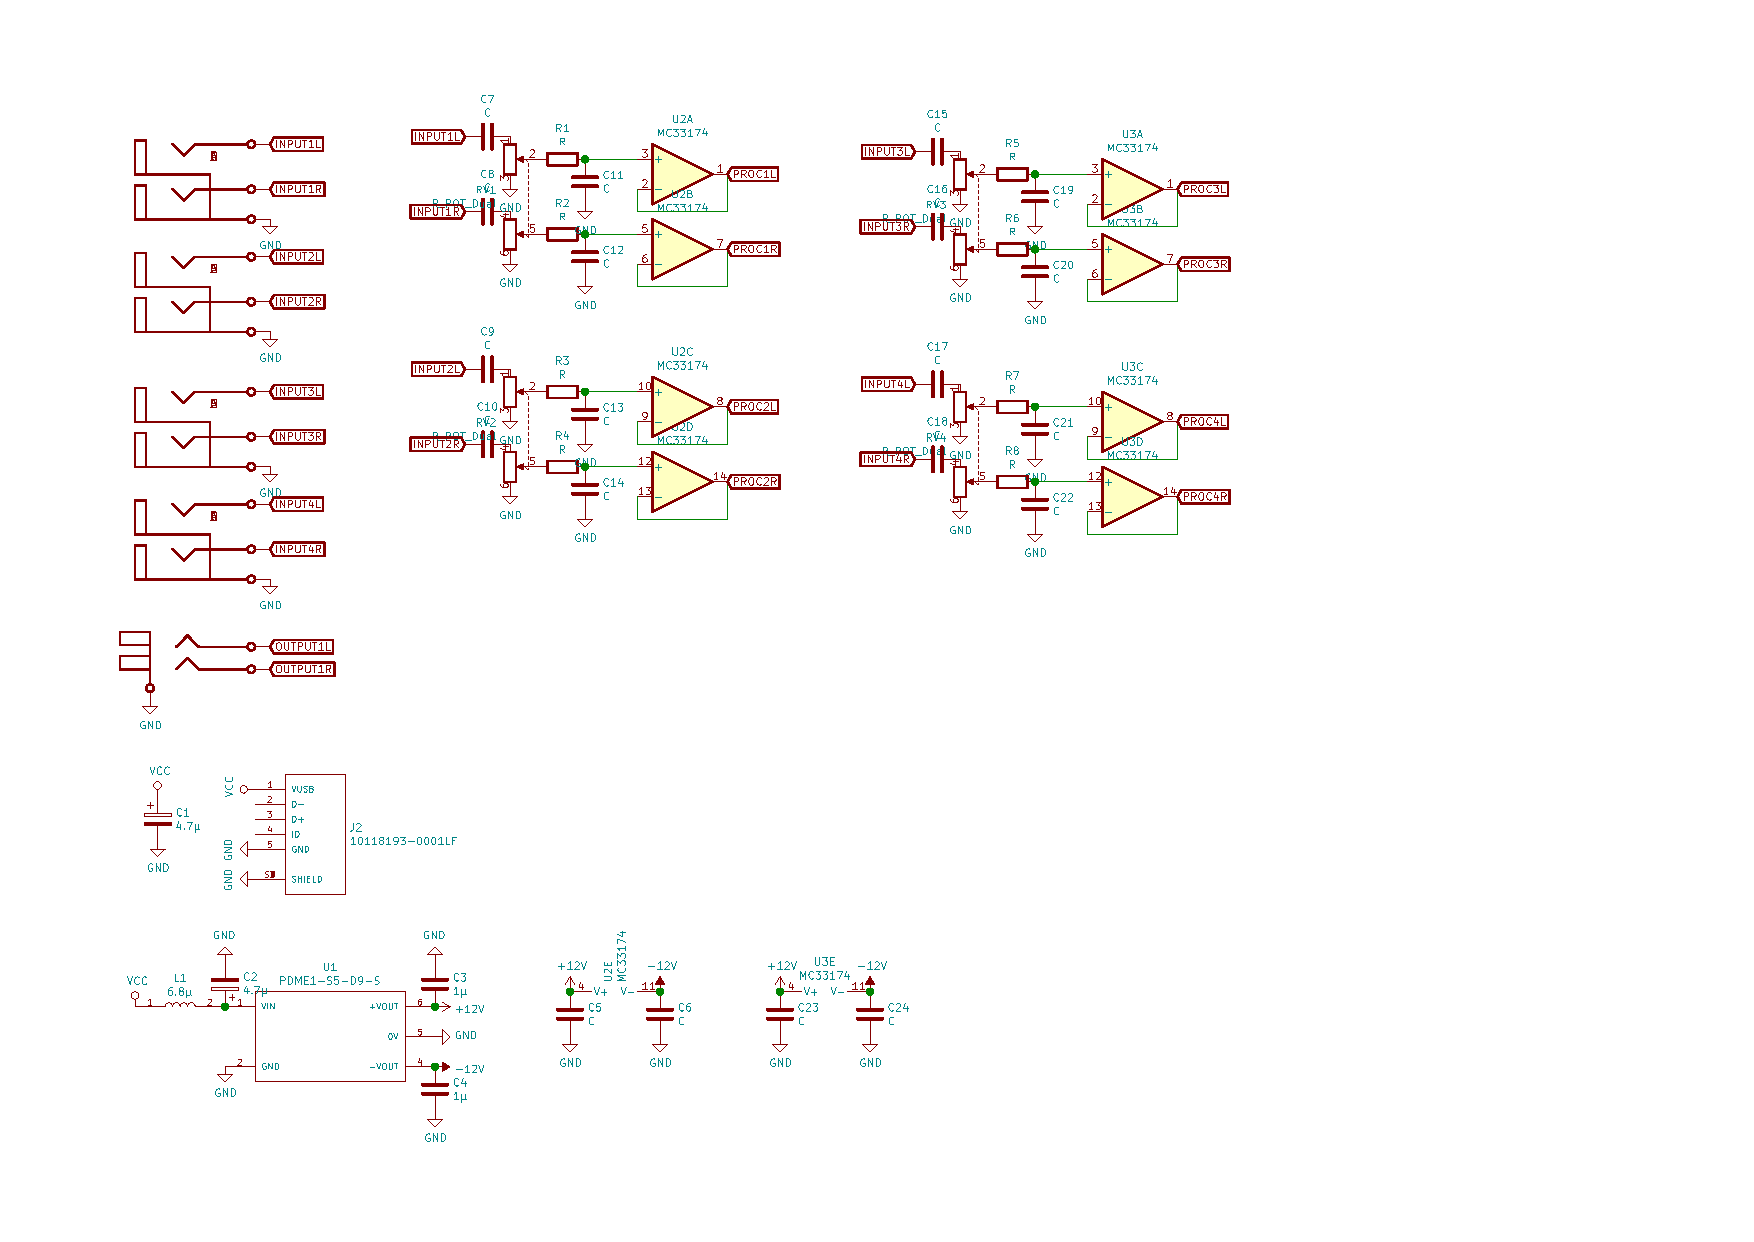
\includegraphics[trim={2cm 10.5cm 24cm 6.2cm},width=4cm,clip]{images/audio-mixer.pdf}
\end{center}

Likewise, I created an instance of the output jack in the schematic and set it up with the proper ground and labels.

\begin{center}
  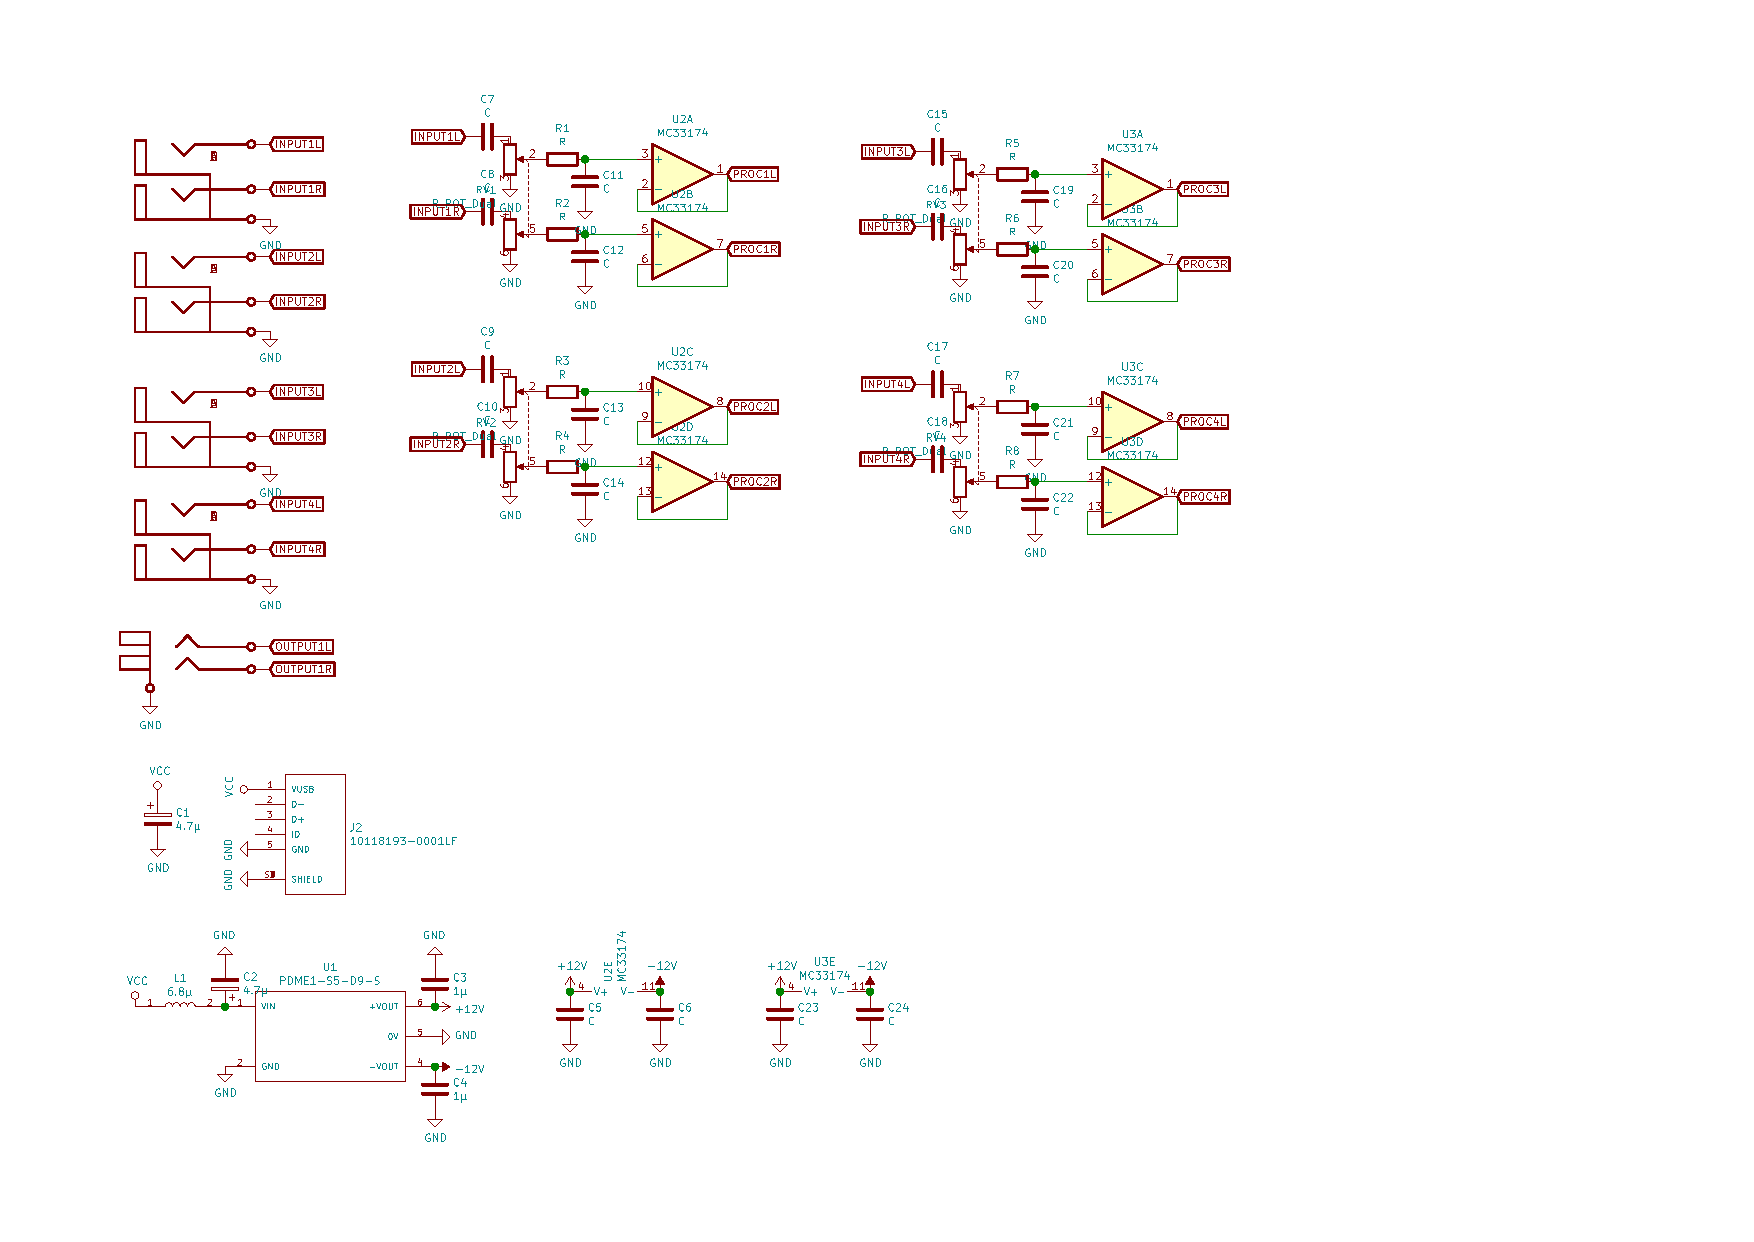
\includegraphics[trim={2cm 8.5cm 24cm 10.4cm},width=4cm,clip]{images/audio-mixer.pdf}
\end{center}

I have found the labels feature to be quite useful to prevent having to route excessive amounts of wires in the schematic, it helps keep things clean.

\subsection{DC to DC Power}

Next I designed the DC to DC Power stage. In this stage, I need to convert the ~5V from the USB into a ±9V or ±12V power rail used by the opamps. The reason I want a range like this is that the opamps will be used to make voltage followers, so they need to have a power rail that is in the range of the signal (which is ±2V line level). It is always good to leave a bit of a margin just to be sure. Also, the opamps don't work too great too close to the rails.

\begin{figure}[h!]
\centering
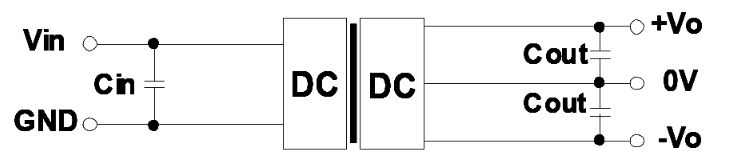
\includegraphics[width=6cm]{images/pdme-dual}
\caption{DC to DC converter dual rail setup}
\label{fig:pdme-dual}
\end{figure}

I first looked at the datasheet provided by the DC to DC converter, which has recommendation on how to use it in a circuit. Figure \ref{fig:pdme-dual} and \ref{fig:pdme-emc} show how the datasheet recommends setting it up, and this is what I followed.

\begin{figure}[h!]
\centering
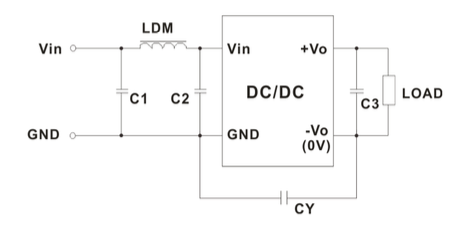
\includegraphics[width=7cm]{images/pdme-emc}
\caption{DC to DC converter EMC recommendation}
\label{fig:pdme-emc}
\end{figure}

The sample circuits are a little confusing, but I just implemented both of them as I thought it makes sense. I did omit CY from Figure \ref{fig:pdme-emc} -- the device supports isolated outputs, but I chose to hook the output up to the ground, making the capacitor there redundant.

\begin{center}
  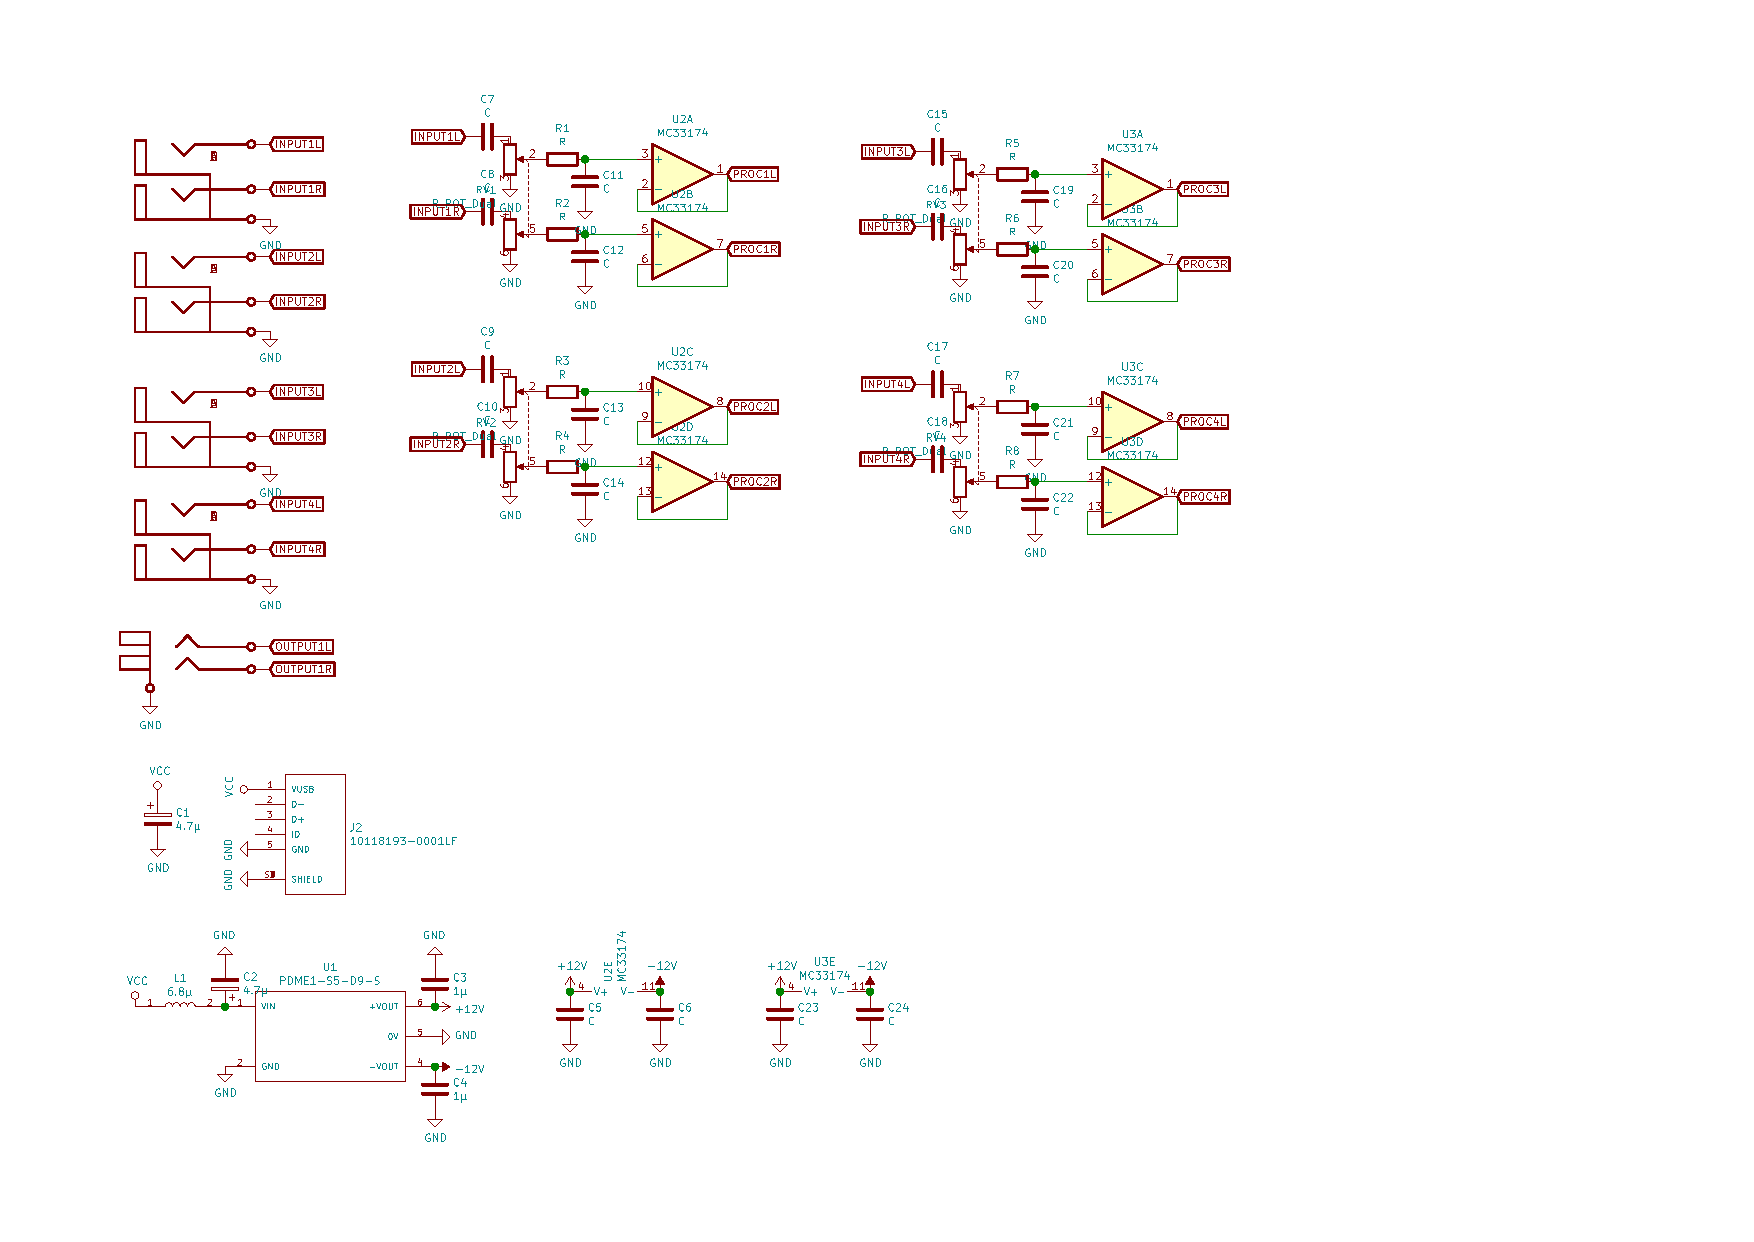
\includegraphics[trim={2cm 1.5cm 21cm 16cm},width=8cm,clip]{images/audio-mixer.pdf}
\end{center}

This is the result that I came up with. Note that the first capacitor, C1 in Figure \ref{fig:pdme-emc}, is not visible -- this can be seen on the USB Power Input side of things. I have labelled the two new power rails +12V and -12V, to differentiate from the existing V\textsubscript{cc} and GND rails.

\subsection{Audio Volume Adjustment}

\subsection{Audio Mixing}


\section{Bill of Materials}

After having done the research on the parts that I will use, the next step is to create a BOM list that helps me understand and break down the cost of the product so far, and helps me find out what I need to source. A lot of parts have multiple possible sources.

\begin{center}
\begin{tabular}{@{}lllll@{}}
\toprule
Part & Description & Count & Unit Price (€) & Price (€)\\
\midrule
SC1537-ND & 8 RCA Jacks & 1 & 3.79 & 3.97\\
102-5864-ND & 2 RCA Jacks & 1 & 1.08 & 1.08\\
497-1597-1-ND & Opamp & 5 & 0.37 & 1.85\\
609-4616-1-ND & Micro USB Connector & 1 & 0.38 & 0.38\\
102-6321-ND & DC to DC Converter & 1 & 2.15 & 2.15\\
P2J4103-ND & Potentiometer & 5 & 1.19 & 5.95\\
& PCB & 1 & 5.00 & 5.00\\
\midrule
Total & & 14 && 20.38\\
\bottomrule
\end{tabular}
\end{center}

My calculations show that the product will cost about 25€ in parts. There is obviously more cost for me, because this does not include shipping. At this time, it also does not include the cost of the case. However, I am happy with that price so far. 

\section{Layout of PCB and Routing}

After I have the schematics and all parts set, I proceeded to do the actual PCB. At first, I just imported all of the parts from the schematic. Then, I placed some rulers to measure a 100 by 50mm square area that would be the size of my PCB. Next, I drew the outlines of this area on the Edge.Cut layer.

Next, I arranged the parts on the PCB in a way that makes sense. The RCA jacks and USB Power Input all went on the same long edge. I spread out the components a bit, such that they were all placed with space around them for laying out connections.

\begin{center}
  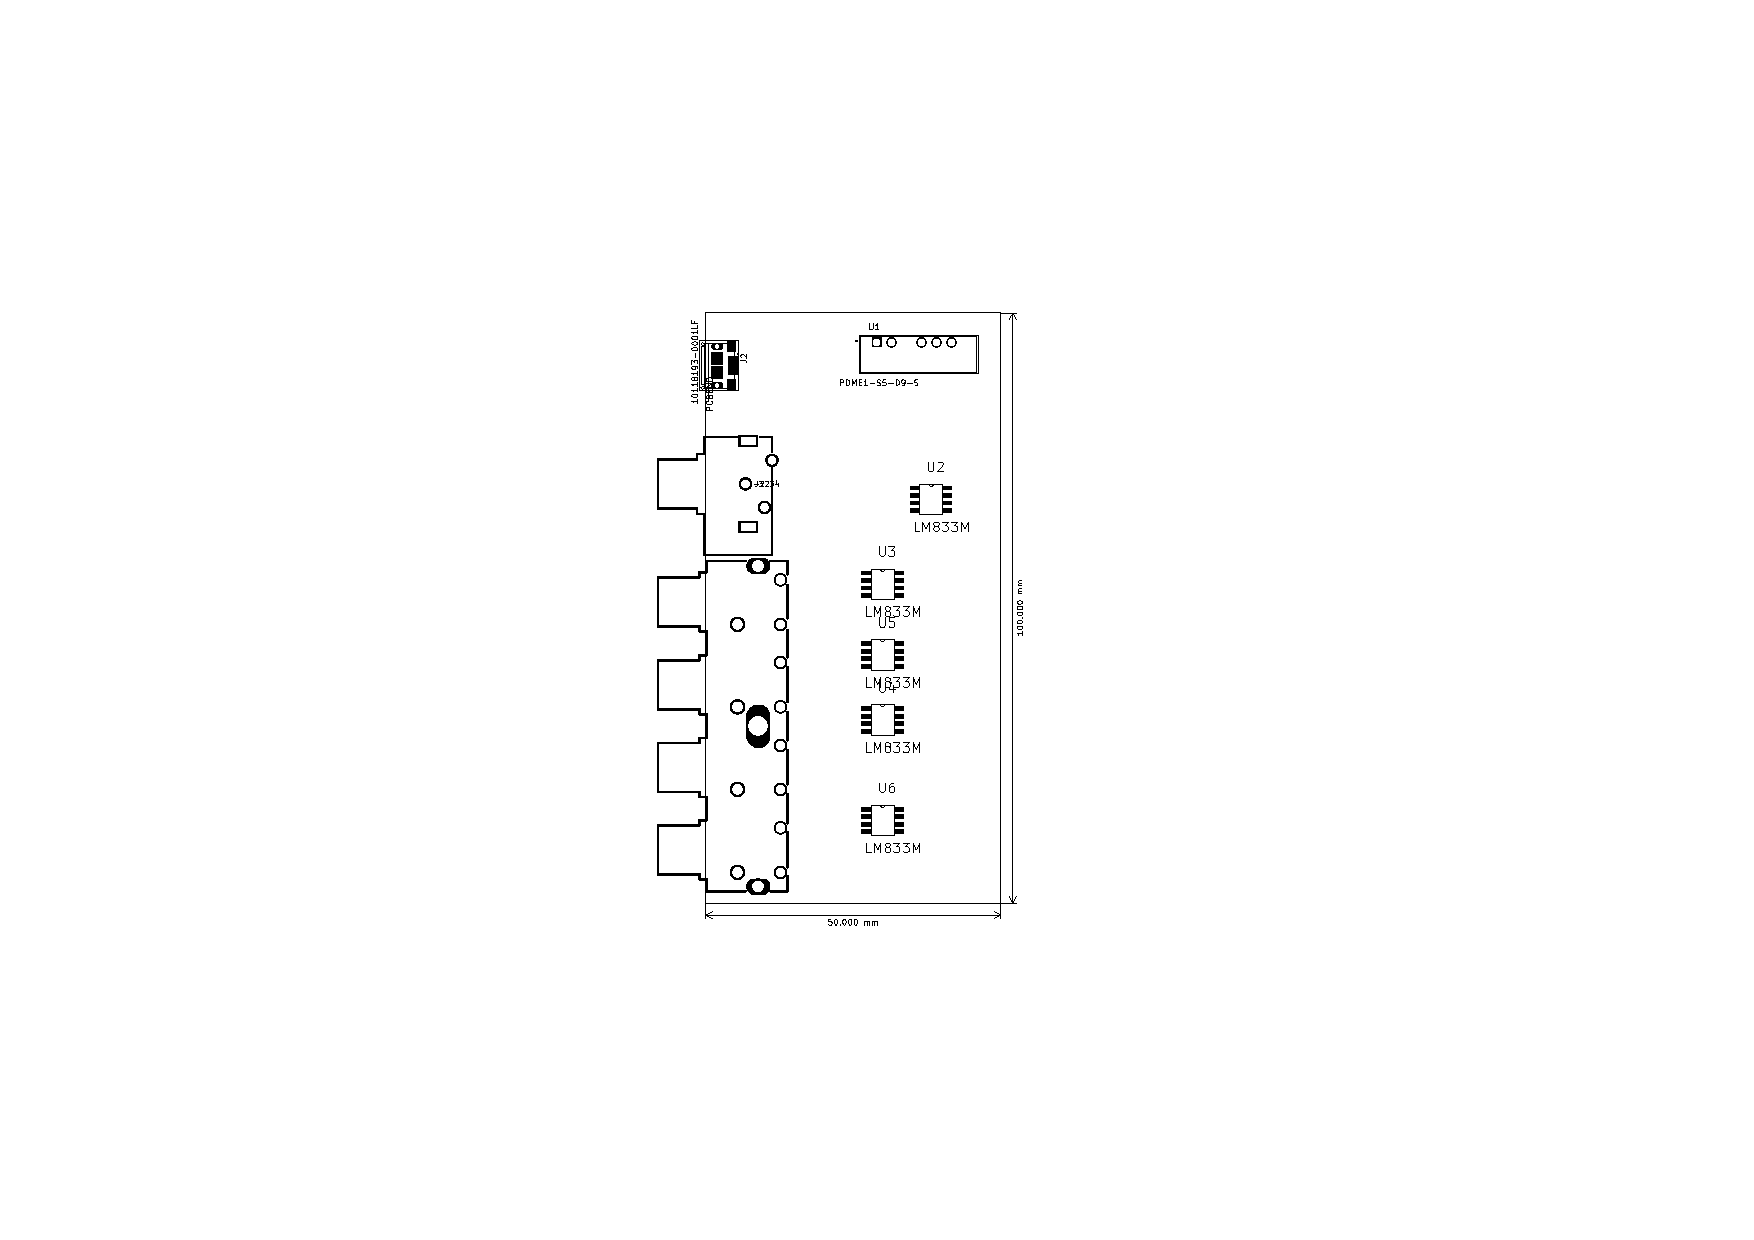
\includegraphics[trim={11cm 5cm 12cm 5cm},clip,width=6cm]{images/pcb.pdf}
\end{center}

I was still missing some outlines and some parts. 


\end{document}